%Victor
\section{Suite de protocole}

\subsection{ARP} ARP (Address resolution protocol) est un protocole à cheval
entre la couche 2 et la couche 3 permettant de faire la conversion entre les
adresses de niveau 2 et de niveau 3. Il fut décrit dans le RFC 826\cite{url-RFC-ARP}.
Il est très utilisé étant donné que les hôte connaissent souvent les adresses
IP de leur destinataire, mais rarement l'adresse de niveau 2 de ce destinataire
ou de la passerelle à contacter pour joindre le destinataire.

\subsubsection{Cache ARP} Le cache ARP ou table ARP est une table sotcké en
local par un hôte et qui ressence les associations entre adresse IP et adresse
MAC.  Ces associations peuvent être soit de type statique, donc écrite "en dur"
par l'administrateur, ou dynamique, donc issue d'échange de trame ARP, et qui
possèdent, en plus des associations statique, une durée de validité, étant
donné qu'une interface peut changer d'adresse IP et qu'il vaut maintenir la
table à jour.  Cette table peut donc être représenté comme une suite d'entrés,
contenant chacune une adresse IP, une adresse MAC et éventuellement une durée
de vie.

\subsubsection{Entête}
//TODO


\subsubsection{Fonctionnement} Prenons l'exemple où A veux envoyer un message à
B. A connait l'adresse IP de B. Donc A va préparer son paquet qu'il va envoyer
à B, avec son adresse IP en source et l'adresse IP de B en destination. La
paquet passe dans la couche liaison, il va être enpaqueté dans une trame de
niveau 2. Cette trame aura comme adresse source l'adresse de niveau 2 de A,
mais à ce moment il ne peux pas completé l'adresse destination de la trame: en
effet, il ne connait l'adresse de niveau 2 du destinataire. La paquet reste
bloqué en couche 2 et ne peux pas être envoyé au destinataire. Comment obtenir
l'adresse de niveau 2 du destinaire?  Le protocole ARP est capable de faire
cette translation.

Pour faire cela l'hôte A va tout d'abord regarder dans sa table ARP si il n'a
pas une entrée pour l'adresse IP à laquelle il souhaite envoyer son paquet. Si
il tourve une correpondance, il va utiliser l'adresse MAC stocker en
correspondance avec l'adresse IP recherché.  Si il ne trouve pas de
correspondance il va emmetre une trame ARPREQUEST pour tenter de contacter le
possesseur de l'adresse IP qu'il souhaite contacter. Il va mettre dans cette
trame (en plus de l'entête de niveau 2) un entête ARP. Celui-ci contient
plusieurs informations:
//TODO quels info mettre? type de trame ARP: request ou reply
Les informations importantes pour permettre la résolution d'adresse sont les
adresses IP source et destination, ainsi que les adresses MAC source et
destination.  L'hôte A va donc mettre son adresse IP en IP source (entête ARP)
et son adresse MAC dans l'adresse physique source (entête ARP). Dans le champ
d'adresse IP destination (entête ARP) l'hôte A va mettre l'adresse IP de l'hôte
qu'il veut contacter. Etant qu'il cherche à avoir l'adresse physique de l'hôte
B, il ne peut pas indiquer d'adresse MAC dans le champ d'adresse physique
destinataire. Ce champ est donc rempli avec la valeur 0.  Sachant que l'hôte A
n'a pas l'adresse physique du destinataire, il va envoyer sa trame en broadcast
pour espérer atteindre l'hôte B sans connaitre son adresse MAC.  Une fois que
l'hôte B reçoit la requète ARP, il va analyser son entête et remplir sa table
ARP avec l'adresse IP de l'hôte A et l'adresse physique de A. Cela permet de
créer une correspondance entre l'adresse IP et MAC de A, pour non seulement
pouvoir répondre à sa requête ARP, et pour pouvoir contacter A dans le futur
sans avoir besoin de refaire la demande ARP.  Ensuite l'hôte B va répondre avec
une trame ARPREPLY. L'entête est similaire aux ARPREQUEST, seul le champ
indiquant s'il s'agit d'une trame ARPREQUEST ou ARPREPLY change. Dans cette
trame, l'hôte B va placer son adresse IP dans le champ adresse IP source et son
adresse physique dans le champ d'adresse physique source. Il va aussi mettre
l'adresse IP de A dans le champ adresse IP destination et l'adresse MAC de A
dans le champ d'adresse physique destination. Il va ensuite envoyer cette trame
en unicast à A.  Lorsque A reçoit la trame ARPREPLY, il va à son tour mettre
dans sa table ARP, la correspondance entre l'adresse IP source et l'adresse MAC
source de la trame (soit les adresses de B).  Une fois cette association mise
en place, le paquet IP que voulait envoyer A au début et mis en pause le temps
que le protocole ARP fasse l'association, est enfin envoyé étant donné que A à
maintenant l'adresse physique de B.

//TODO ARP REPLY en broadcast

\subsubsection{ACD} Le protocole ACD (Adresse conflict detection) permet, comme
son nom l'indique, de détecter les conflits d'adresse, qui sont l'utilisation
de la même adresse IP par deux ou plusieurs hôtes en même temps. Pour ce faire
il utilise le protocole ARP avec une succession d'étape permettant de garantir
l'utilisation de manière unique d'une adresse IP. Il fut décrit dans le RFC 5227\cite{url-RFC-ACD}.

Pour commencer, ACD intervient au moment où une interface reçoit une adresse IP
(soit par DHCP, soit par une configuration manuelle,...). Il faut à ce moment vérifier si
l'adresse proposer n'est pas déjà utlisé par un autre hôte sur le réseau.
L'hôte va alors émettre une requète ARP en broadcast en remplissant l'entête
ARP avec son adresse MAC dans le champ d'adresse physique source et 0.0.0.0
dans l'adresse IP source (car il n'a pas encore d'adresse IP attribuer, et pour
éviter de corrompre les table ARP des autre hôte). Le champ adresse IP
destinataire est complété avec l'adresse que l'on souhaite acquérir. On ne peut
pas remplir le champ d'adresse physique destinataire étant donné qu'on ne sait
pas si il y a des hôte avec cette adresse déjà configuré.  Une requète ARP
contenant 0.0.0.0 comme adresse IP source est appelé ARP probe car elle sert à
"sonder" si un autre hôte utilise déjà l'adresse que l'on passe dans le
l'adresse IP destinataire.

Après avoir attendu un temps pouvant aller jusqu'à 1 seconde, l'hôte va envoyer
un nombre d'ARP probe compris entre 1 et 3, et tous espacé d'un intervalle
compris entre 1 et 2 secondes.  Si dans un délai de 2 secondes après l'émission
de l'ARP probe l'hôte reçoit un paquet ARP request ou reply avec comme adresse
IP source l'adresse qu'il souhaite acquérir, alors cela veut dire qu'un autre
hôte est entrain d'utiliser cette adresse. L'ARP reply peut être la réponse à
l'ARP probe émis et l'ARP request peux simplement être une demande ARP faite
par l'hôte qui utilise déjà l'adresse que l'on souhaite acquérir.  En plus de
surveiller ces deux types de messages, l'hôte doit vérifier les message ARP
probe qu'il reçoit. En effet, il se peut que deux hôte décide de configurer
leur interfaces avec la même adresse au même moment. Sachant qu'aucune de ces
deux interface n'a encore d'adresse IP attribuer, aucune ne va répondre à l'ARP
probe deu deuxième hôte. Cela va conduire à l'attribution de la même adresse
pour plusieurs interfaces. Pour éviter ce problème l'hôte doit surveiller les
ARP probe qui passe à son interfaces. Si il en reçoit un avec comme adresse
destination la même adresse qu'il souhaite acquérir mais avec une adresse
physique différente de la sienne, cela veux qu'un autre hôte souhaite utiliser
la même adress que lui. Dans ce cas l'adresse ne peut pas être utilisé de manière sûr.

Si après les 2 secondes d'attente du dernier ARP probe, l'hôte n'a pas reçu d'ARP probe,
ou d'ARP request/reply indiquant un conflit d'adresse, alors l'hôte peut considérer que
l'adresse qu'il souhaite utilisé est unique dans le réseau, et qu'il peut l'utiliser de
manière sûr.

La dernière étape est d'annoncer que l'hôte utilise l'adresse qu'il vient d'acquérir.
Pour ce faire l'hôte va émmettre en broadcast deux ARP Announcement à 2 secondes d'intervalles.
Ces messages sont semblable à des ARP probe à la seul différence que l'adresse IP source
et destination sont l'adresse que vient d'acquérir l'hôte.
Le but étant de créer une entré dans la table ARP des autre hôtes sur le réseau avec l'adresse
que vient d'acquérir l'hôte avec son adresse MAC. Cela permet d'assurer que les autres hôtes
auront bien la nouvelle adresse MAC associer à l'adresse IP au cas où celle-ci était attribué à
une autre interface dans le passé.


Dans un deuxième temps, ACD va être utilisé en permanence durant l'utilisation d'un adresse IP
dans la mesure où lorsque que la l'interface va recevoir un paquet ARP, elle va analyser
si l'adresse IP source correspond à une de ces adresses, et si cela est la cas et que l'adresse
MAC ne correspond à son adresse MAC, alors cela veut dire qu'un autre hôte utilise la même
adresse IP. Il y a donc un conflit d'adresse.
Pour résoudre ce problème, l'hôte peut réagir de différente manière:
\begin{itemize}
\item Il cesse d'utiliser l'adresse IP en question.
\item Si l'hôte doit pour quelque raison que ce soit garder son adresse IP, par exemple si il
utilise une connection TCP, alors il peut "défendre" sa possession de l'adresse IP, seulement si
il n'a pas reçu d'autre paquet ARP portant à conflit dans les 10 dernières seconde.
Il va pour cela noter le temps auquel il a reçu le paquet posant un conflit d'adresse et émettre un ARP Announcement en donnant son adresse MAC en association avec
l'adresse IP. Il va envoyer ce paquet à son adresse IP, pour signaler à l'hôte qui utilise
aussi cette adresse qu'il y a un conflit d'adresse. Cependant il peut y avoir une boucle sans
fin si les deux hôtes utilisant la même adresse se renvoient mutuellement un ARP Announcement
pour défendre son adresse. Pour éviter ce scénario, si plusieurs paquet ARP posant un conflit
d'adresse sont détecté dans les 10 dernières secondes (d'où l'importance de noter le temps où l'hôte à reçu les paquets posant problème), alors l'hôte cesse d'utiliser son adresse
pour éviter de rentrer dans une boucle sans fin d'échange d'ARP Announcement.
\item Si l'hôte à été configurer pour garder son adresse IP (par exemple si c'est un routeur
ou un serveur) alors l'hôte va défendre son adresse indéfiniment. //TODO compléter
\end{itemize}


\subsection{ICMP} ICMP (Internet Control Message Protocol) est un protocole de
niveau 3 faisant partie intégrante du protocole IPv4. Il fut initialement
décrit dans le RFC 792\cite{url-RFC-ICMP}.
Il permet de transmettre des informations de controle et d'erreur. Les messages
ICMP sont empaquetés dans des paquets IP, ils diposent donc d'un entête de
paquet IP. Cet entête est le même que pour tout les autres entêtes de paquet
d'IPv4. Deux champs sont intéressant dans le cas d'un paquet ICMP, les champs
Protocol et Type of service. Le champ Protocol est mis à à la valeur 1 pour
dire que le paquet contient un message ICMP, et le champ ToS est mis à 0
//TODO(pourquoi 0?)//.  Après le header du paquet IPv4, commence la partie data
//qui contient le message ICMP. Ce message contient des champs différent en
//fonction du type de message à passer. Cependant les trois premier champs sont
//toujours les mêmes.


\begin{figure}
\centering
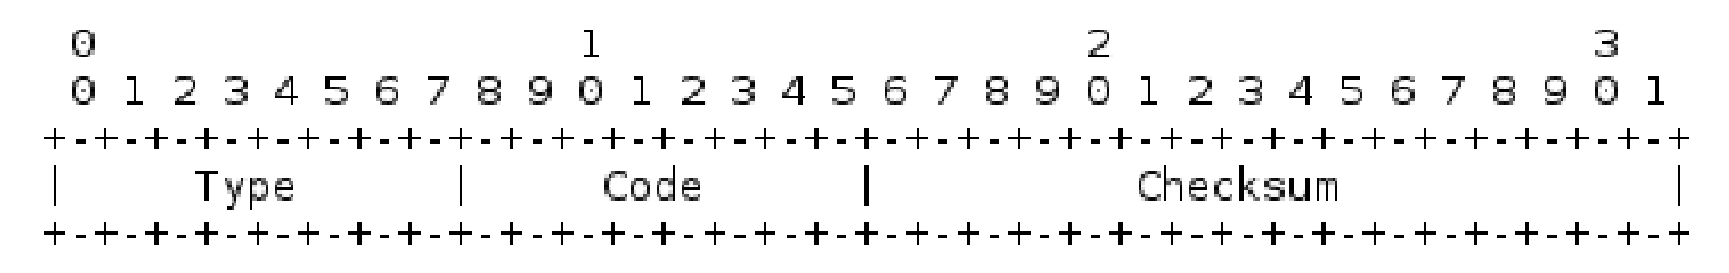
\includegraphics[width=15cm]{./pics/header.eps}
\caption{TODO}
\label{fig:headicmp}
\end{figure}

Le premier champ est celui de type. Il permet, premièrement, de donner le type
du paquet et de l'information à transmettre, et deuxièmement de préciser la
nature des champs qui vont suivres. En effet, comme vu plus haut, les messages
contiennent des champs différents selon le type du message ICMP.
Le deuxième champ est le code. Il permet de subdiviser le type en donnant des détails plus
précis. Enfin le troisième champ est la somme de contrôle
(checksum)//TODO(plage de controle).  Commençons avec les messages qui
possèdent l'ensemble de champs le plus simple.

\begin{figure}
\centering
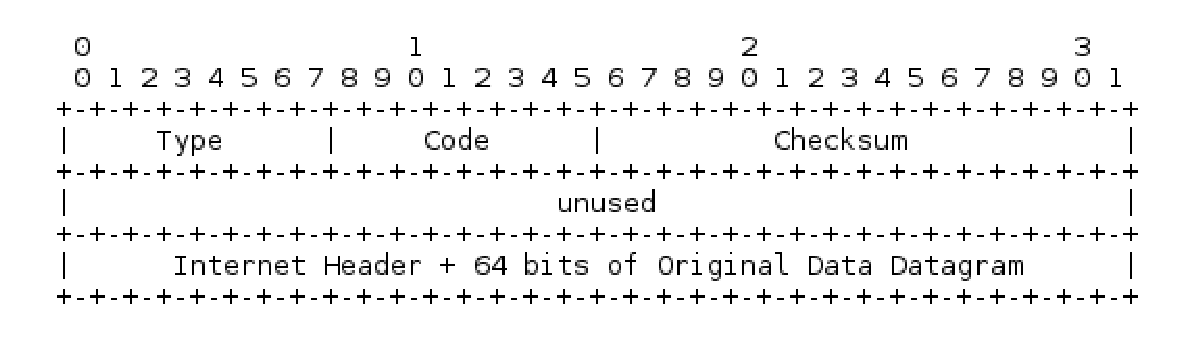
\includegraphics[width=15cm]{./pics/header1.eps}
\caption{TODO}
\label{fig:head1icmp}
\end{figure}

Les messages qui utilisent cette organisation sont les messages de type 3, 4
et 11.
Le champ Internet header contient l'entête du paquet qui a été supprimé plus
les 64 bits suivant celui-ci. Cela permet à l'émetteur de retrouver quel paquet
à été supprimé.


\subsubsection{Message de type 3: Unreachable Destination}
Les messages de type 3 sont émis lorsqu'un paquet n'a pas réussi à joindre la
destination (Unreachable destination). Cette erreur peux être dut à plusieurs
facteurs, et les codes permettent de préciser pourquoi le paquet n'a pas pu
rejoindre sa destination.

\paragraph{Code 0: Network Unreachable} Ce code indique que le réseau qu'un hôte essaye
d'atteindre n'est pas joignable; ceci étant dut à l'absence de route vers ce réseau.

\paragraph{Code 1: Host Unreachable} Ce code indique que le réseau à été joint, mais que
le routeur sur ce réseau n'arrive pas à joindre l'hôte à qui délivrer la trame.

\paragraph{Code 2: Protocole Unreachable} Ce code indique que l'hôte à été joint, mais
que le protocole utilisé //TODO quel protocole de quel niveau?// n'est pas actif.

\paragraph{Code 3: Port Unreachable} Ce code indique que l'hôte à été joint, mais que le
port utilisé en couche transport n'est pas actif et ne peux donc être utilisé pour
communiquer.

\paragraph{Code 4: Fragmentation needed} Ce code indique que la taille du paquet dépasse
le MTU (Maximum Transmission Unit) et que le flag DF à été mis dans l'entête IP.
En règle général, si un paquet est plus grand que le MTU, il doit être fragmenté par le
routeur pour être transmis en plusieurs paquets plus petit. Mais comme le flag DF (Do not
Fragment), le paquet ne peux être fragmenté. Le routeur emet donc un paquet ICMP de code 4.

//TODO quel autre code?



\subsubsection{Message de type 4: Source Quench Message}
//TODO PLus utulisé, est ce qu'on en parle?

\subsubsection{Message de type 11: Time Exceeded}
Ces messages sont envoyés lorsque le TTL d'un paquet à atteind 0. Une autre
utilisation des ces messages est lorsque que le temps de ré-assemblage des
fragments d'un paquet est dépassé. Ces deux cas sont distingé par le code. Ces
messages ont pour destinataire l'hôte qui à envoyé le paquet qui à provoqué
l'erreur.//TODO(vérifier).

\paragraph{Code 0:}
Le code 0 est utilisé pour indiquer que le TTL du paquet posant problème est arrivé à 0.
Lorsque le TTL d'un paquet arrive à 0, celui-ci est supprimer et un message
ICMP de type 11 et de code 0 est envoyer par le routeur qui à détécté le
problème. Cela permet principalement d'éviter qu'un paquet sans dans une boucle
et qu'il soit rélayé à l'infini.

\paragraph{Code 1:} Le code 1 est quant à lui utilisé pour indiquer que l'hôte n'a pas
réussi à réassembler les fragments du paquet IP original dans la limite de temps prévue
à cet effet.


\subsubsection{Message de type 5: Redirect Message} Les message de type 5 utilisent les entêtes
ci-dessous et servent à faire de la redirection. En effet, lorsqu'un routeur
détecte que le prochain routeur dans lequel va transiter le paquet se trouve
dans le même réseau que l'émetteur de ce paquet, il va envoyer un message ICMP
pour avertir cet hôte (et/ou le réseau) qu'il existe un chemin plus court en
envoyant directement les paquets vers le prochain routeur. Ce message ICMP va
avoir pour effet de modifier la table de routage interne à l'émetteur (et/ou
des hôtes connecté au réseau). Concernant le paquet que le premier routeur à
reçu, il va le transmettre vers sa destination.


\begin{figure}
\centering
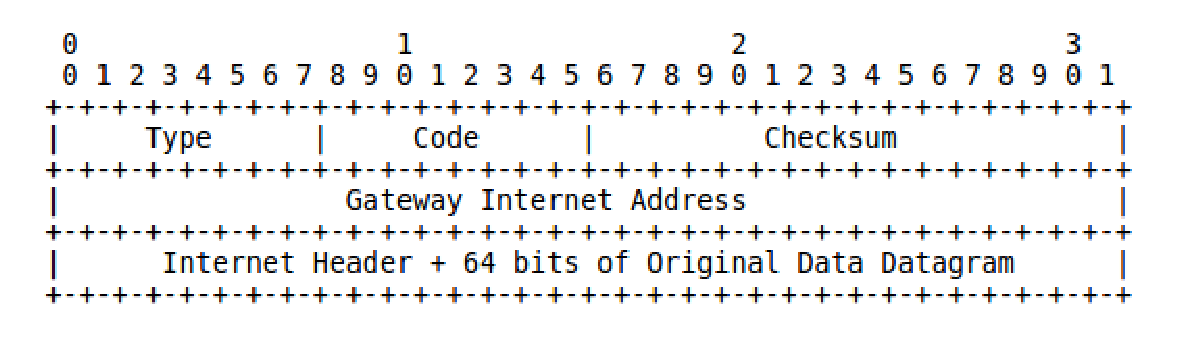
\includegraphics[width=15cm]{./pics/header2.eps}
\caption{TODO}
\label{fig:head2icmp}
\end{figure}
Le champ Gateway Internet Address contient la l'adresse du routeur auquel il
faut faire transiter le traffique directement pour avoir un chemin de routage
plus court.  Le champ Internet Header contient toujours l'entête du message
ayant porvoqué l'envoie du message ICMP plus les 64 bits suivant l'entête. Cela
permet à (aux) hôte(s) de pouvoir modifier leur table de routage en fonction la
destination que cherchait à atteindre le paquet.

\paragraph{Code 0}
Ce code indique que la redirection est adresser à tout le réseau de l'émetteur du
paquet.

\paragraph{Code 1}
Ce code indique que la redirection est adresser à l'émetteur du paquet.

\paragraph{Code 2}
Ce code indique que la redirection est adresser à tout le réseau de l'émetteur
du paquet et aux services(//TODO(préciser)).

\paragraph{Code 3} Ce code indique que la redirection est adresser à l'émetteur
du paquet(//TODO(préciser)).

\begin{figure}
\centering
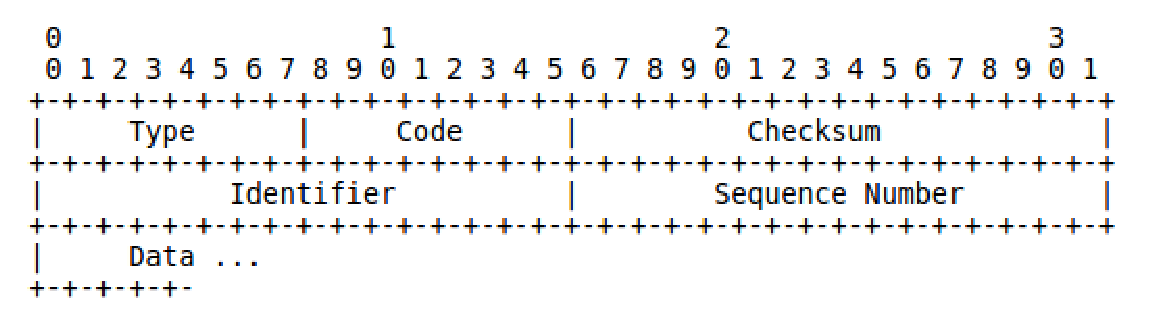
\includegraphics[width=15cm]{./pics/header3.eps}
\caption{TODO}
\label{fig:head3icmp}
\end{figure}

\subsubsection{Message de type 8 et 0: Echo Request et Reply} Les messages de type 8 et 0 servent à
faire des envoies et des renvoies d'information. Ils utilisent pour cela
l'entête ci-dessus. Les messages de type 8 font des envoies d'informations,
appelé echo request. Tandis que les messages de type 0 sont envoyés en réponse
aux echo request et renvoie les informations reçus de ceux-ci; ils sont appelés
echo reply. Etant donnée que les echo reply sont des réponses aux echo request,
l'adresse destination des echo reply est l'adresse source des echo request. Ces
deux messages peuvent être envoyés et reçus aussi bien par un hôte que par un
routeur. Ce sont notamment les message envoyés par la commande {\it ping} qui
permettent de vérifier si l'on peux communiquer avec un hôte ou un routeur.  Les
champs Identifier et Sequence Number aide l'émetteur de l'echo request à
associer les echos request qu'il à envoyés avec les echos reply qu'il à reçus.
//TODO(qui a t-il dans data?)

\subsection{IGMP}
Le protocole IGMP est un autre protocole faisant partit intégrante d'IPv4. Il permet en effet aux hôtes
de communiquer aux routeur mutlicast leur abonnement à des groupes multicast.
IGMPv2 et IGMPv3 sont les versions les plus utilisées actuellement. Elles sont
respectivement décritent dans le RFC 2236 et RFC 3376.
Les messages IGMP sont divisées en trois groupe:
\begin{itemize}
\item Membership Query: Les requètes d'adhésion: servant aux routeurs pour faire
une demande aux hôtes des groupes auxquels ils abonnés.
\item Membership Report: Les rapports d'hôte sur leurs abonnements.
\item Leave Group: Message annoncant l'arrêt d'un abonnement d'un hôte.
\end{itemize}
Tout ces messages sont envoyés avec un TTL de 1, pour éviter que ceci ne passent
d'un réseau à un autre.

IGMP va donc permettre aux routeurs d'apprendre les groupes d'abonnements des hôtes qui
sont sur le réseau ou les réseaux du routeur.
Le routeur dispose d'une liste des groupes multicast auxquels les hôte d'un réseau sont connectés,
et ceci pour tout les réseaux auxquels il est connecté.
Pour commencer, le routeur va envoyer à l'adresse 224.0.0.1, 2 Membership Query général
(par défaut) à 30 secondes d'intervalles (par défaut).

Lorsqu'un hôte reçoit un Membership Query, il va initialiser un timer pour chaque
groupe multicast auxquels il appartient. Ces timers sont initialiser avec un temps
aléatoire dont la borne supérieur est spécifié dans le Membership Query. Ce système
de timers permet de ne pas saturer le réseau avec touts les message IGMP de tout les
groupes qui seraient envoyé au même moment.
Lorsque le timer d'un des abonnements arrive à 0, alors l'hôte émet, en multicast au
groupe en question, un Membership Report.
Si l'hôte reçoit un Membership Report et que le timer du groupe concerné par le
message reçus n'a pas encore atteind 0, alors l'hôte va arrêter le timer. En effet le
routeur sera aux courant de l'existance du groupe car il a reçu le même rapport que
l'hôte.
Le protocole IGMP est conçu pour que le routeur sache à quels grouep multicast sont
abonner les hôte sur les réseaux auxquels il est relié. Cependant le protocole n'a pas
du tout été conçu dans l'optique de fournir la liste des hôtes avec leurs abonnements.
C'est pour cela qu'une fois que le routeur est au courant de l'existence d'un groupe,
les autre hôtes faisant partit de ce groupe n'envoie pas de rapport pour ce groupe.

Lorsque le routeur reçoit un Membership Report il va ajouter le groupe à sa liste de groupe
présent sur le réseau auquel il est connecté. Il va à ce moment initialiser un timer
à 135 secondes (valeur par défaut).
Si il reçoit d'autre Membership Report pour un groupe existant alors le timer est
remis à sa valeur initiale.
Lorsqu'un hôte rejoint un nouveau groupe, il va emmettre un Unsolicited Membership Report
pour s'annoncer dans le groupe, et ainsi informer le routeur de l'éxistence de ce groupe
ou de la remise à la valeur initiale du timer.

Le dernier cas de figure est cas où un hôte veut se désabonner d'un groupe. Si l'hôte
est le dernier de son groupe alors il va envoyer un Leave Group à l'adresse 224.0.0.2.
Si il n'est pas le dernier, il peux simplement ne rien faire et se désabonner du groupe,
il ne sera pas plus concerné par les messages à destination du groupe. Etant donné qu'il
y a d'autres membres dans le groupe ceci s'occuperont de "maintenir le groupe en vie".
En revanche si l'hôte ne sais pas si il est le dernier hôte dans le groupe rien ne l'empêche
d'envoyer un Leave Group.

Lorsque le routeur reçoit un Leave Group, il sais qu'un membre à quitté le groupe. Ce qui
l'intéresse est de savoir si il y a encore des membres dans le groupe en question ou
si s'est le dernier membre qui vient de quitter le groupe. Il va pour cela envoyer deux
Membership Query spécifiquement au groupe en question. Si aucune réponse n'est reçut en
réponse le groupe est considéré comme n'ayant plus de membre et il est oublier du routeur.
Si jamais les hôte n'annonçait pas leur retrait du groupe (comme cela à été évoqué plus haut)
et qu'il n'y avait plus d'hôte faisant partit du groupe, alors le groupe serait considéré
sans membre et oublier lorsque le timer du routeur arriverai à 0 pour le groupe en question.

Le dernier point pour que tout cela fonctionnent, est qu'il faut que le routeur envoie
régulièrement des Membership Query général pour qu'il maintiennent à jour sa table des
groupe présent sur le réseau, sinon ceux-ci serait oublier une fois le timer arrivé à expiration.

\subsection{DHCP}
Le protocole DHCP (Dynamic Host Configuration Protocol) sert à l'autoconfiguration
des interfaces. Plus précisement, il  permet d'attribuer une adresse IP à une
interface et de lui faire parvenir d'autres information essentielle pour le
fonctionnement de l'interface sur le réseau. La version initiale de DHCP fut décrit
dans le RFC 1531\cite{url-RFC-DHCP1}, mais cette version fut rendue obselète par un autre
RFC, lui même rendue obselète par le RFC 2131\cite{url-RFC-DHCP2} qui est la dernière version non
obselète.Voyons comment une interface peut ce configurer aurpès d'un serveur DHCP.

\begin{figure}
\centering
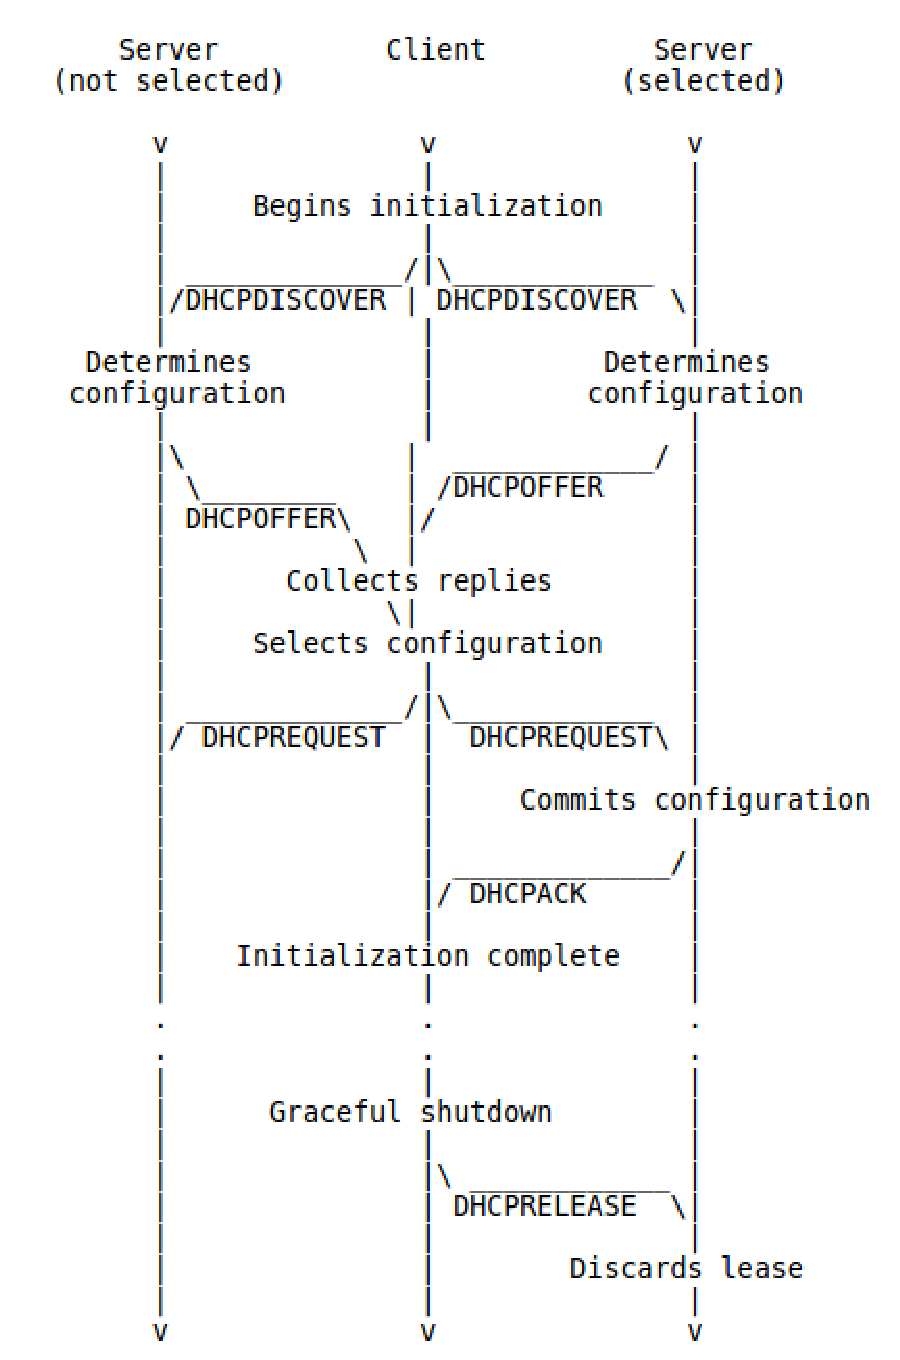
\includegraphics[width=6cm]{./pics/timeline_dhcp.eps}
\caption{TODO}
\label{fig:timelinedhcp}
\end{figure}

Lorsqu'une interface, qui n'a pas d'adresse IP, souhaite en recevoir une, elle
va emettre un message DHCPDISCOVER en broadcast sur son réseau. Des agents DHCP
peuvent faire passer
ce message DHCP sur un autre réseau si le serveur DHCP (qui distribue les
adresses) ne se trouve pas sur le même réseau que l'hôte qui fait la demande.
L'hote va utiliser comme adresse IP 0.0.0.0.

Etant donnée que le message est envoyé en broadcast, tout les hôtes sur le
réseau vont recevoir le message, et en particulier le ou les serveurs DHCP qui
pourraient s'y trouver. Si cela est le cas, ceux-ci vont répondre avec un
DHCPOFFER. Ce message contient entre autre l'adresse IP proposé pour le client
souhaitant se configurer, ainsi que le masque de sous-réseau de l'adresse. A ce
moment là l'adresse n'est pas encore attribuer et réservé pour l'hôte étant
donnée qu'il peux refuser l'offre et accepter l'offre d'un autre serveur. Si
jamais l'hôte ne reçoit aucun DHCPOFFER, il va ré-émettre un DHCPDISCOVERY. Si
il reçoit un ou plusieurs DHCPOFFER, l'hôte va devoir choisir une configuration
qui lui est proposé. Une fois ce choix fait, il va informé les serveurs DHCP de
son choix à l'aide d'un message DHCPREQUEST émis en broadcast. Ce message va
contenir l'identifiant du serveur DHCP retenu ainsi que la configuration
souhaité par l'hôte (adresse IP et masque de sous-réseau). Ce message peut être
interprété de deux manières différentes selon le serveur:
\begin{itemize}
\item si ce n'est pas le serveur retenu, il considère le message comme une
déclinaison de l'offre.

\item si c'est le serveur retenu, il va sortir l'adresse attribué l'hôte de la
plage d'adresse libre pour ne plus l'attribuer à un autre hôte. Il va ensuite
émmetre un message DHCPACK contenant la configuration effective de l'hôte avec
notemment: l'adresse IP, le masque de sous-réseau, la durée du bail, l'adresse
de la passerelle par défaut et l'adresse du serveur DNS.  Si pour quelque
raisons le serveur n'est pas capable d'attribuer l'adresse proposé dans l'offre
(par exemple si l'adresse à été attribuer entre temps), le serveur emet un
DHCPNAK pour avertir l'hôte que l'adresse n'est plus disponible. L'hôte devra
alors recommencer la procédure pour obtenir une adresse IP.
\end{itemize}

Enfin si le serveur ne reçoit pas de message DHCPREQUEST, la procédure
s'arrêtrra à ce moment et l'adresse n'étant pas encore attribuer à l'hôte elle
reste disponible pour être attribuer à d'autre hôte.  Arrive la dernière étape.
Si le client reçois un message DHCPACK, il peux prendre en compte la
configuration (adresse IP, masque de sous-réseau, DNS, passerelle par défaut et
durée de bail). Il va effectuer une dernière vérification pour s'assurer que
l'adresse qui lui à été attribué est bien unique sur le réseau pour éviter
d'avoir deux hôte avec la même adresse. Il va pour cela utilisé le protocole
ARP et la méthode de vérification vu plus haut. Si jamais l'adresse est déjà
utilisé par un autre hôte, il va envoyer un message DHCPDECLINE au serveur DHCP
pour lui indiquer qu'il n'utilisera pas la configuration proposé par celui-ci,
et il va recommencer la procédure pour pouvoir obtenir une nouvelle
configuration.

Si jamais l'adresse proposé par le serveur est unique sur le réseau, la
configuration est terminé et l'hôte peut utiliser l'adresse (durant la durée du
bail de celle-ci).  Dernier cas possible, si jamais le l'hôte ne reçoit pas de
DHCPACK ou de DHCPNAK, il va réemettre le message DHCPREQUEST pour esperer
recevoir une réponse du serveur.

//TODO algo de retransmission TODO fonctionnement agent relais dhcp client peut
//renoncer à son bail identification des message faisant partit d'un meme
//echange avec client identifier, server identifier TODO fonctionnement bail

L'hôte est donc configuré et peut utiliser son adresse. Cependant, il ne peut
l'utiliser que durant la durée de son bail. Une fois le bail expiré, l'hôte ne
peux plus utiliser son adresse. Lorsque l'hôte à reçu le message DHCPACK du
serveur, celui-ci lui a transsmis la durée du bail. De cette durée, l'hôte va
en extraire deux temps noté T1 et T2. T1 correspond à la moitié de la durée du
bail et T2 à 0.875 la durée du bail. Ces temps sont exprimé de manière relatif
étant donnée que les horloges du serveur et de l'hôte ne sont pas
synchronisées.  Une fois que l'hôte à atteind le temps T1, il va chercher à
contacter le serveur qui lui à attribué sa configuration avec un message
DHCPREQUEST pour étendre la durée de son bail. Ce message est émis de manière
unicast. A ce moment l'hôte est entré en état RENEWING. Si l'hôte reçoit un
message DHCPACK du serveur lui accordant un prolongement de la durée de son
bail, alors il va sommer le temps qu'il avait insérer dans le DHCPREQUEST avec
la durée accordé par le serveur et qui se trouve dans le message DHCPACK.
L'hôte retourne dans l'état BOUND. Cependant l'hôte n'est pas obligé d'attendre
T1 pour pouvoir étendre son bail.  Si jamais l'hôte ne reçoit pas de reponse
DHCPACK avant l'arrivé de T2, il passe en état REBINDING. A ce moment il va
émettre un DHCPREQUEST en broadcast pour espérer pourvoir étendre son bail
auprès de n'importe quel serveur DHCP. Pour parer aux eventuels cas de perte de
DHCPREQUEST, l'hôte va renvoyer un message une fois la moitié de la durée entre
T1 et T2 passé, en état RENEWING; et une fois la moitié de la durée entre T2 et
la fin du baille , en état REBINDING(et avec un minimum de temps de 60
secondes).  Si malgré tout, la durée du bail venait à expirer, alors l'hôte ne
possèderait plus de configuration réseau et ne pourrait plus communiquer avec
d'autre hôtes. Il rentre alors en état INIT; il doit alors recommencer la
procédure pour obtenir une adresse configuration.

Cependant,dans ce cas comme dans d'autre, l'hôte peut ré-utiliser une
configuration précédement utilisée. Cela permet de raccourcir la négociation
entre l'hôte et le serveur DHCP. L'hôte va directement commencé la négociation
en faisant un DHCPREQUEST en broadcast et contenant la configuration qu'il
souhaite ré-utiliser. Le serveur concerné par l'attribution antérieur de la
configuration va donc accepter la demande de l'hôte à l'aide d'un DHCPACK ou la
refuser, si la demande n'est pas correct ou si l'adresse est utilisé par un
autre hôte, à l'aide d'un DHCPNAK.  Cette négociation se fait de manière
similaire qu'un négocation complète, elle a juste été raccourci en enlevant
quelque étape non indispensable.

\begin{figure}
\centering
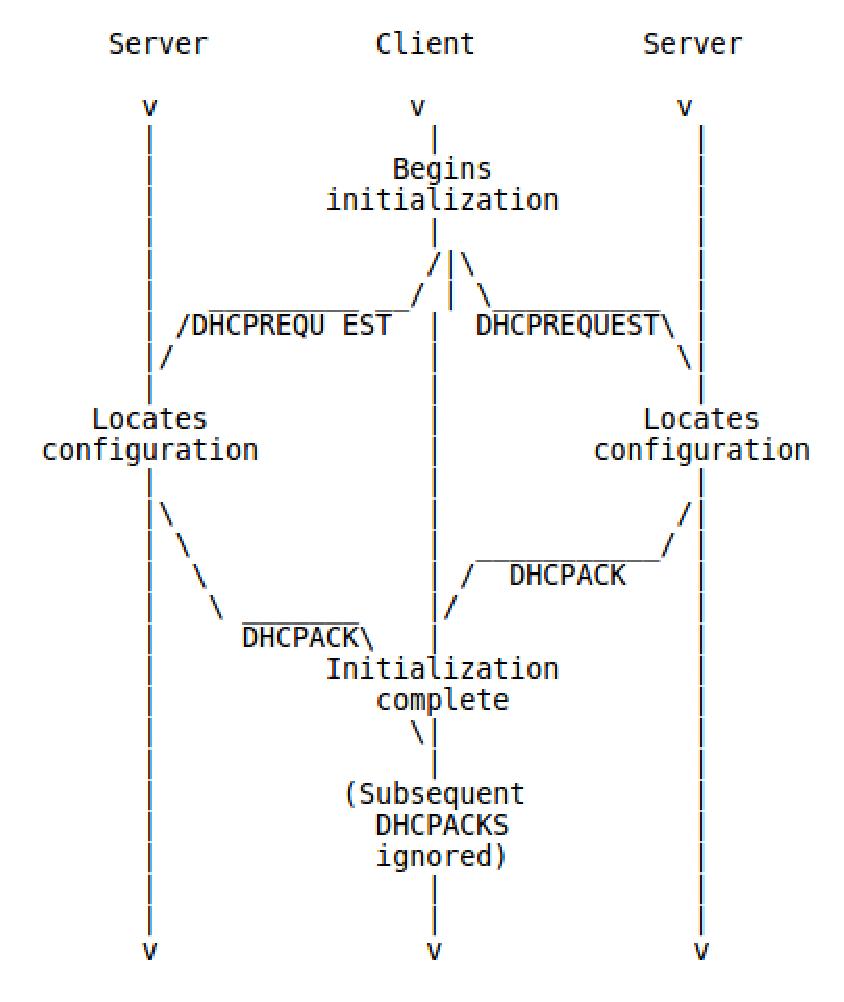
\includegraphics[width=6cm]{./pics/timeline_dhcp_reuse_add.eps}
\caption{TODO}
\label{fig:timelinedhcpreuseadd}
\end{figure}

\subsection{PMTU discovery}
Le protocole PMTU discovery (Path MTU discovery) décrit dans le RFC 1191\cite{url-RFC-PMTU}, permet de trouver le plus petit MTU d'un chemin entre l'émetteur et le récepteur. Cela permet d'éviter la fragmentation des paquet IP ce qui permet entre autre de soulagé la charge des routeurs.
L'hôte souhaitant connaitre le plus petit MTU pour un chemin vers autre hôte va envoyer un paquet avec un certain MTU et en plaçant le bit DF de l'entête sur DF, pour éviter la fragmentation du paquet. Ainsi si le MTU est trop grand à un moment donné du chemin, le routeur ne pourra pas fragmenter le paquet mais ne pourra non plus pas transmettre le paquet en l'état. Il va alors détruire le paquet, et émettre un message ICMP de type 3 et de code 4 à la source, signalant que la destination n'est pas joignable, et que cela est à un paquet nécessitant une fragmentation. Mais la fragmentation est interdite pour ce paquet. Le MTU est donc trop élevé. Le message ICMP contient le MTU qu'il faut passé le routeur.
L'émetteur va alors créer un nouveau paquet avec le nouveau MTU. Il fera cela autant de fois que cela est nécessaire pour déterminer le MTU du chemin.

\subsection{DNS}
Le protocole DNS (Domain Name System) permet de faire de la résolution d'adresse.
Cela permet grâce à des échange entre un ou plusieurs serveur DNS de faire la traduction
de nom de domaine, notamment en adresse IP. Pour simplifier, le nom de domaine, facilement
retenable pour un être humain va être traduit en adresse IP pour être utilisé par l'ordinateur.
Nous n'aborderons pas plus le fonctionnement de DNS car s'est un protocole de couche application
et qu'il n'est pas essentielle au fonctionnement d'IPv4. Cependant il reste essentielle dans
l'utilisation d'Internet, aujourd'hui, par des êtres humains.
